%!TEX root = ../template.tex
%%%%%%%%%%%%%%%%%%%%%%%%%%%%%%%%%%%%%%%%%%%%%%%%%%%%%%%%%%%%%%%%%%%%
%% chapter5.tex
%% NOVA thesis document file
%%
%% Chapter with lots of dummy text
%%%%%%%%%%%%%%%%%%%%%%%%%%%%%%%%%%%%%%%%%%%%%%%%%%%%%%%%%%%%%%%%%%%%

\typeout{NT FILE chapter5.tex}%

\chapter{An approach to automate the modeling class diagrams}
\label{cha:approachAutomateModeling}
In this chapter, we describe the design, configuration, and integration of our automated class diagram modeling system. 
Section \ref{sec:promptTechniqueAndModelUsed} details the process of selecting the most suitable prompt technique and large language model (LLM) for the task, supported by empirical evaluation. 
Section \ref{sec:RAGSystemImplemented} presents the construction and optimization of the Retrieval-Augmented Generation (RAG) pipeline, including the embedding models, text splitters, retrievers, and vector store configurations tested. 
Section \ref{sec:selfImproveApproach} introduces the self-refinement mechanism, explaining its iterative evaluation–improvement loop and prompt engineering strategies. Section \ref{sec:systemArchitecture} outlines the architecture of the complete system, integrating generation, refinement, and rendering modules into a coherent workflow. 
Section \ref{sec:automatic_modelation_pipeline} describes the automated modeling pipeline, detailing the steps from input processing to diagram generation. 
Section \ref{sec:challenges} discusses the main challenges faced during development, including cost control and RAG component selection, and the strategies adopted to overcome them. 
Finally, Section \ref{sec:praticalDemonstration} provides a practical demonstration of the system applied to a realistic use case, comparing the AI-generated class diagram to the ground truth and drawing conclusions from the results.

\section{Prompt technique and Model used}
\label{sec:promptTechniqueAndModelUsed}
From the expirement present on the previous chapter (/ref{Experiments with prompt techniques and different LLM models}) we shaw that claude offered the most balanced performer, having the best G-eval results, adding to the fact the models provided to anthropic have shown great results in software engineering tasks, as it can be seen in the SWE-Leaderboard (https://swe-bench-live.github.io/). We decided to use CoT since was the prompt that achieved the best overall results.

Having selected the prompt and the family of models to use we had to decide which model to use. To help making this decision we conducted a expirement using the same setup used in the previous chapter to evaluate and test the different LLM models and prompt techniques to select which is the best model to use.

From the results we can see that the models had struggle  identifying the attributes and the methods present in the ground truth resulting in a lower recall value(as it can be seen in figure \ref{fig:recall}).  This can be do to the system description not being very clear in some attributes and methods which reconfirms the importance of complete unambiguous system description as it was found in the papers analyze in the state of the art.

\begin{figure}[htbp]
    \centering
    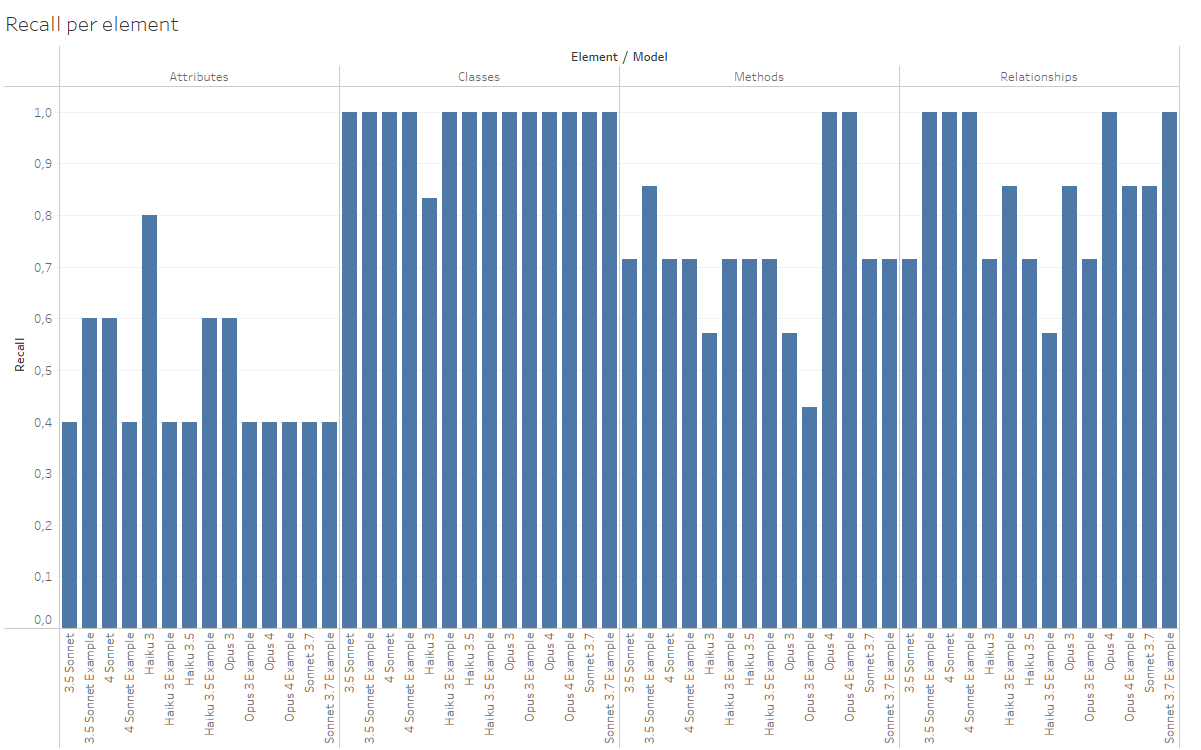
\includegraphics[width=0.6\linewidth]{Chapters/Figures/Recall_per_element.png} % Adjust width or use height
    \caption{ Recall per element of the class diagram }
    \label{fig:recall}
\end{figure}

Since we are going to use Anthropic API every call has a price and that price can go higher if the number of input token is high. Therefore we tested what is the influence of having an example in the prompt. 

To better evaluate the overall performance of the models we calculated a overall score.

\begin{equation}
\resizebox{\textwidth}{!}{$
\text{Overall Score} = \frac{1}{4} \left(
\underbrace{\frac{\text{Validity Score} + \text{Completeness Score}}{2}}_{\text{Semantic quality}} +
\underbrace{\frac{\text{Pragmatic Score} + \text{Pragmatic Clarity Score}}{2}}_{\text{Pragmatic quality}} +
\underbrace{\frac{\text{Syntactic Score} + \text{UML Completeness Score} + \text{UML Quality Score}}{3}}_{\text{Structural UML quality}} +
\underbrace{\text{Requirement Coverage Score}}_{\text{Requirement Coverage quality}}
\right)
$}
\end{equation}

Looking at the overall score we can see that out of the six models five benefit from having an example in the prompt. Reforcing the hipoteses that adding examples to the prompt can improve the result of the LLMs, the results can be seen in the figure \ref{fig:overallScore_Models}. 

\begin{figure}[htbp]
    \centering
    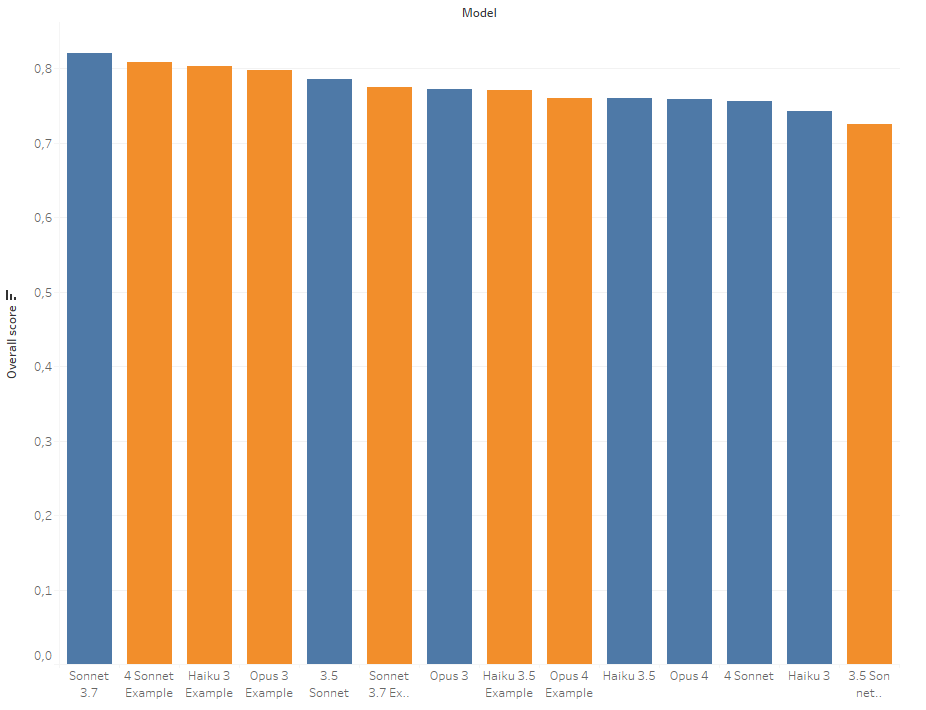
\includegraphics[width=0.6\linewidth]{Chapters/Figures/models.png} % Adjust width or use height
    \caption{ Overall score of the models with and without example in the prompt }
    \label{fig:overallScore_Models}
\end{figure}

We aim to have all the elements present in ground truth diagrams therefore its important that the model that we will be using have a good recall meaning that. Looking at the recall average for each model we can see that the best one 3.5 Sonnet followed by the most powerfull models Opus 4 and Sonnet 4. 3.7 Sonnet also is in the top 4 models present also a good solution.

When deciding the model it is also important to look at the prices and compare the overall performance to price, to do so we calculated the prices of each prompt based on the number of input tokens we were sending and the max output tokens estableshed (2000 tokens).

\begin{figure}[htbp]
    \centering
    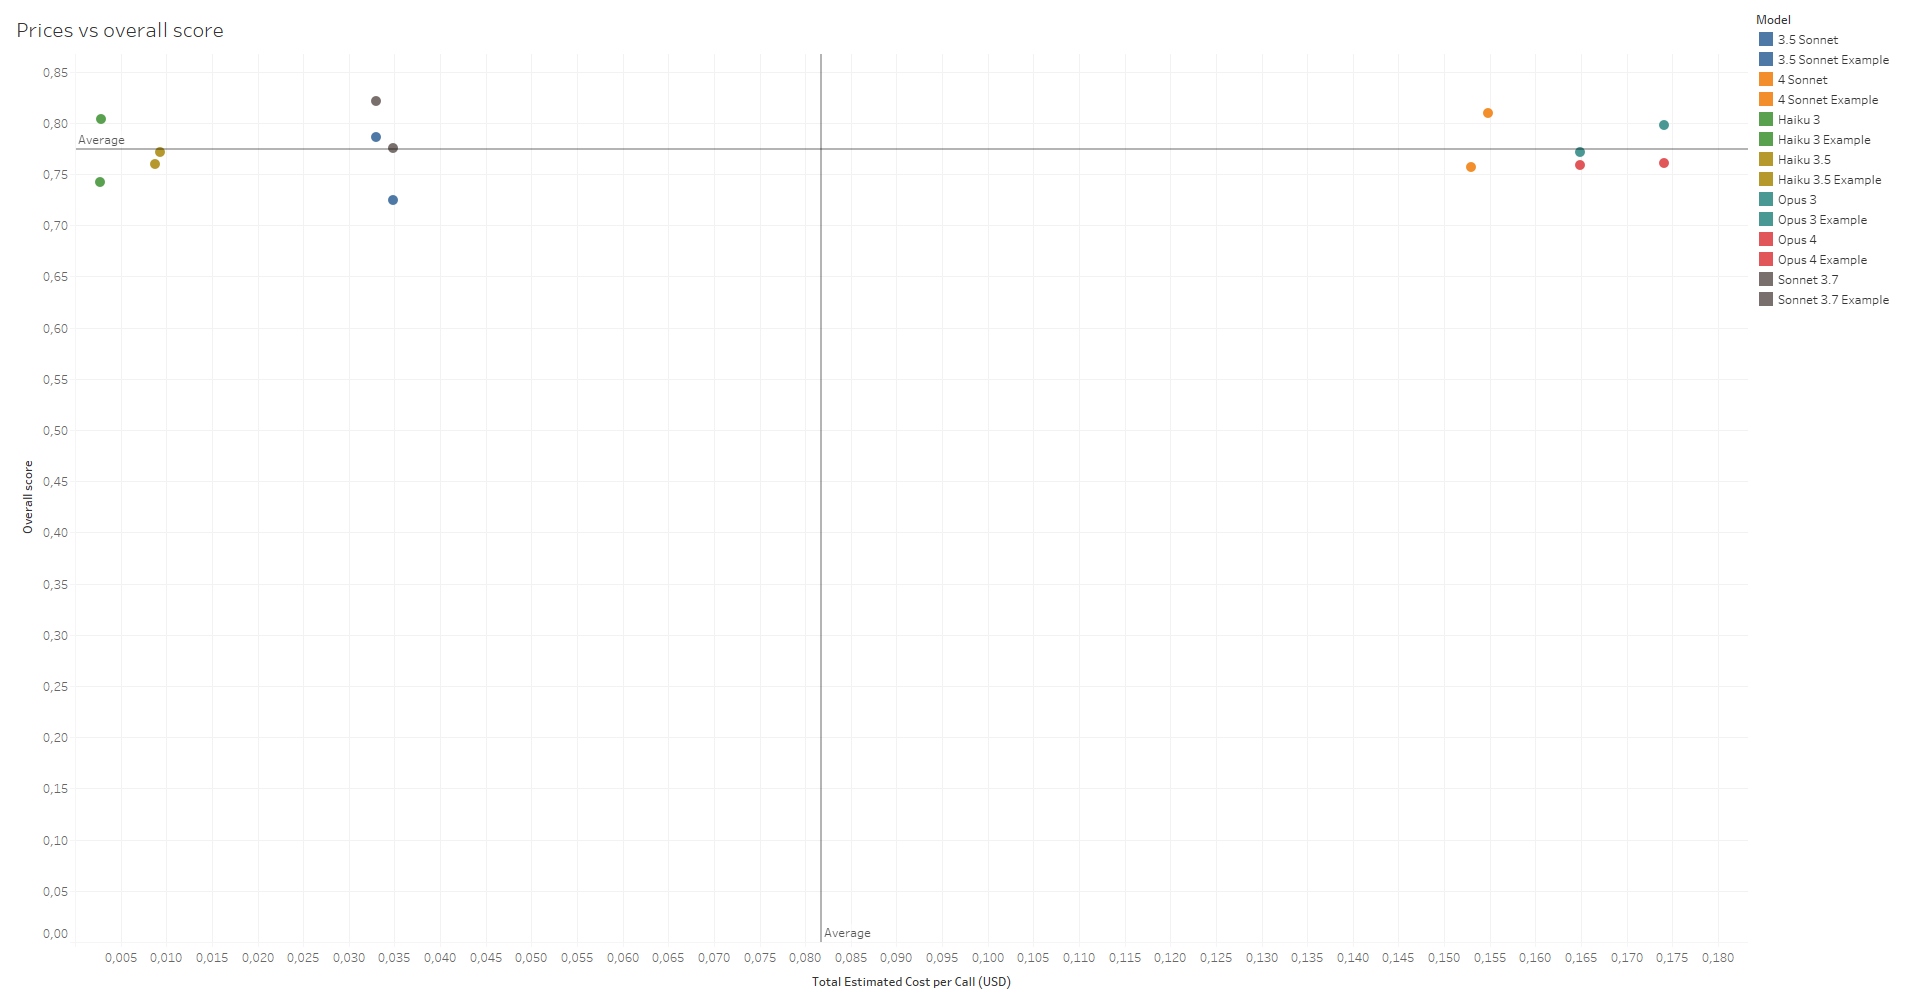
\includegraphics[width=0.6\linewidth]{Chapters/Figures/overall_score_prices.png} % Adjust width or use height
    \caption{ Overall score vs price of the models}
    \label{fig:overallScore_price}
\end{figure}
As seen in the figure \ref{fig:overallScore_price} the best cost-performance model would be present in the second quadrant. There are two models in this second quadrant (Sonnet 3.7, Sonnet 3.5 and Haiku 3).  Sonnet 3.7 has the best score out of the three.
The top two models would be the Sonnet 3.7 and the Sonnet 3.5 for our use case. The Sonnet 3.7 had better overall result then Sonnet 3.5, however Sonnet 3.5 had better F1-score and recall and is cheaper that Sonnet 3.7 per call, therefore we are going use the Sonnet 3.7. However since haiku is almost 12 times cheaper and also had good results we are going to use haiku 3 in testing phase.

\section{Retrieval Augmented Generation System implemented}
\label{sec:RAGSystemImplemented}

After selecting the model and the prompt being used, we proceeded to design and configure our Retrieval-Augmented Generation (RAG) system. Due to time and hardware constraints, we were only able to test a limited number of component combinations. To ensure feasibility, we focused on \textbf{simple and lightweight configurations} that could run efficiently on local infrastructure.

To support this process, we developed a custom script to automate the creation and evaluation of different RAG pipeline configurations. Each configuration was composed by combining embedding models, text splitters, retrievers, and a vector store. We evaluated their performance using \textbf{direct open-ended questions related to UML, PlantUML, and class diagrams}, spanning various levels of difficulty.

Each configuration was assessed based on the following metrics:
\begin{itemize}
    \item Retrieval time
    \item Number of chunks generated
    \item Accuracy
    \item Semantic similarity
    \item Completeness
    \item Relevance
    \item Syntax correctness
    \item Overall score (computed with the following formula):
\end{itemize}

\begin{equation}
\text{Score} = (\text{accuracy} \times 0.25 + \text{semantic\_similarity} \times 0.25 + \text{completeness} \times 0.2 + \text{relevance} \times 0.15 + \text{syntax\_correctness} \times 0.15)
\end{equation}

The different components we tested were:

\begin{enumerate}
    \item \textbf{Embedding models}
    \begin{enumerate}
        \item all-MiniLM-L6-v2
        \item all-mpnet-base-v2
        \item multi-qa-MiniLM-L6-cos-v1
        \item all-distilroberta-v1
        \item paraphrase-multilingual-MiniLM-L12-v2
    \end{enumerate}
    \item \textbf{Text splitters}
    \begin{enumerate}
        \item Recursive text splitter with chunk size = 300 and chunk overlap = 20 (Default)
        \item Recursive text splitter with chunk size = 1024 and chunk overlap = 200 (Large Chunks)
        \item NLTK text splitter with chunk size = 300 and chunk overlap = 20
    \end{enumerate}
    \item \textbf{Retrievers}
    \begin{enumerate}
        \item Similarity with $k = 3$
        \item MMR with $k = 3$ and fetch\_k = 10
        \item Similarity with a score threshold = 0.5 and $k = 10$
        \item BM25
        \item Ensemble (0.5 BM25 and 0.5 vectorstore)
    \end{enumerate}
    \item \textbf{Vector store}
    \begin{enumerate}
        \item Chroma
    \end{enumerate}
\end{enumerate}

The difference between top and bottom configurations is statistically small, suggesting diminishing returns.

\subsection*{Results and Discussion}

Looking at the top 10 overall, all had a score higher than 0.67318, although the difference between top and bottom configurations is statistically small. This suggests \textbf{diminishing returns} and points to the importance of secondary metrics (e.g., speed, semantic quality) when making trade-offs.

The \textbf{best overall configuration} used:
\begin{itemize}
    \item Embedding: \texttt{multi-qa-MiniLM-L6-cos-v1}
    \item Splitter: Recursive (chunk size = 300, overlap = 20)
    \item Retriever: MMR ($k = 3$, fetch\_k = 10)
\end{itemize}

This setup achieved:
\begin{itemize}
    \item \textbf{Overall score} $\approx 0.684$
    \item \textbf{Retrieval time} $\approx 0.044\ \text{s}$
    \item \textbf{Semantic similarity} $\approx 0.567$
    \item \textbf{Accuracy} $\approx 0.631$
    \item \textbf{Relevance} $\approx 0.593$
    \item \textbf{Chunks}: 2580
\end{itemize}

While it produced the \textbf{highest number of chunks}, this was expected due to the small chunk size (300). The higher chunk count contributed positively to retrieval quality, particularly relevance and completeness.

In terms of \textbf{semantic similarity}, this configuration ranked 5th among the top 10. However, since \textbf{semantic similarity and relevance showed no linear correlation} (Pearson $r \approx 0.02$), this metric should be interpreted independently.

The configuration achieved \textbf{second-highest accuracy} among top-ranked results, confirming its robustness across both semantic and factual dimensions.

Regarding \textbf{retrieval time}, this setup was not the absolute fastest but remained well within efficient limits ($<0.05\ \text{s}$). The \textbf{fastest configuration} used \texttt{all-MiniLM-L6-v2} with MMR and the NLTK splitter, achieving $\approx 0.15\ \text{s}$, but with a slightly lower overall score.

\textbf{Chunk count analysis} showed that smaller chunk sizes (e.g., 300) improved performance at the cost of retrieval volume, whereas larger chunks did not improve scores despite reducing memory and time costs.


\begin{figure}[htbp]
    \centering
    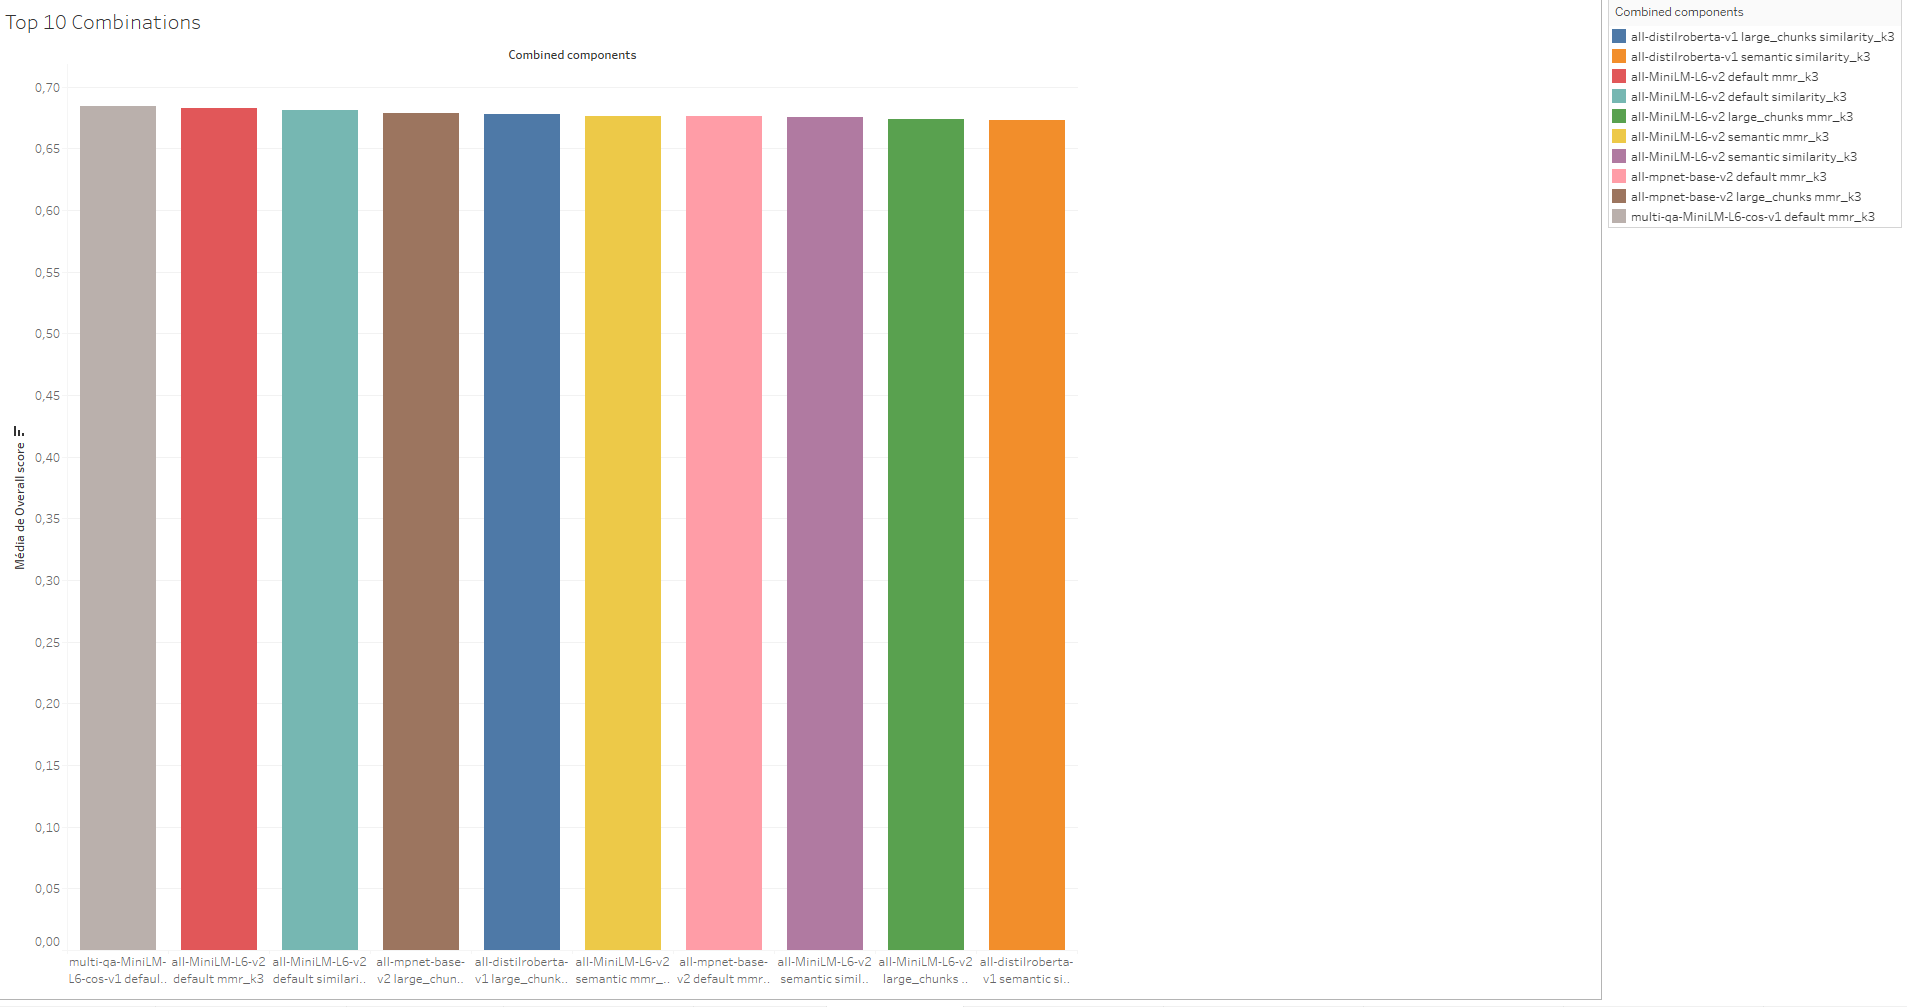
\includegraphics[width=0.6\linewidth]{Chapters/Figures/overall_score_combinations.png}
    \caption{Top 10 configurations}
\end{figure}

\begin{figure}[htbp]
    \centering
    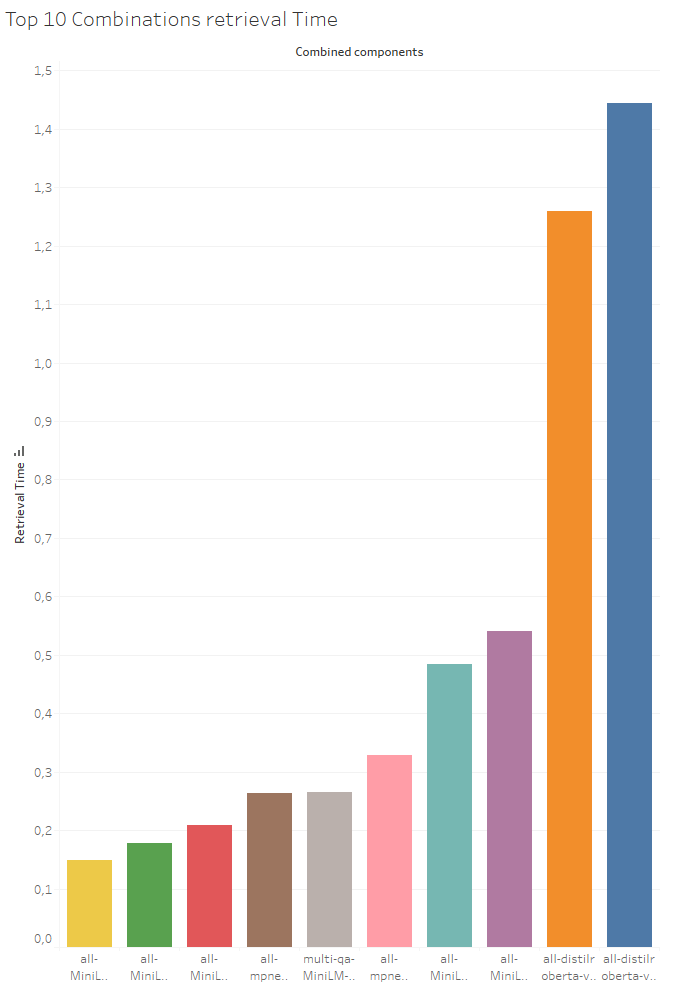
\includegraphics[width=0.6\linewidth]{Chapters/Figures/retrieval time.png}
    \caption{Retrieval time of the top 10 configurations}
\end{figure}

\begin{figure}[htbp]
    \centering
    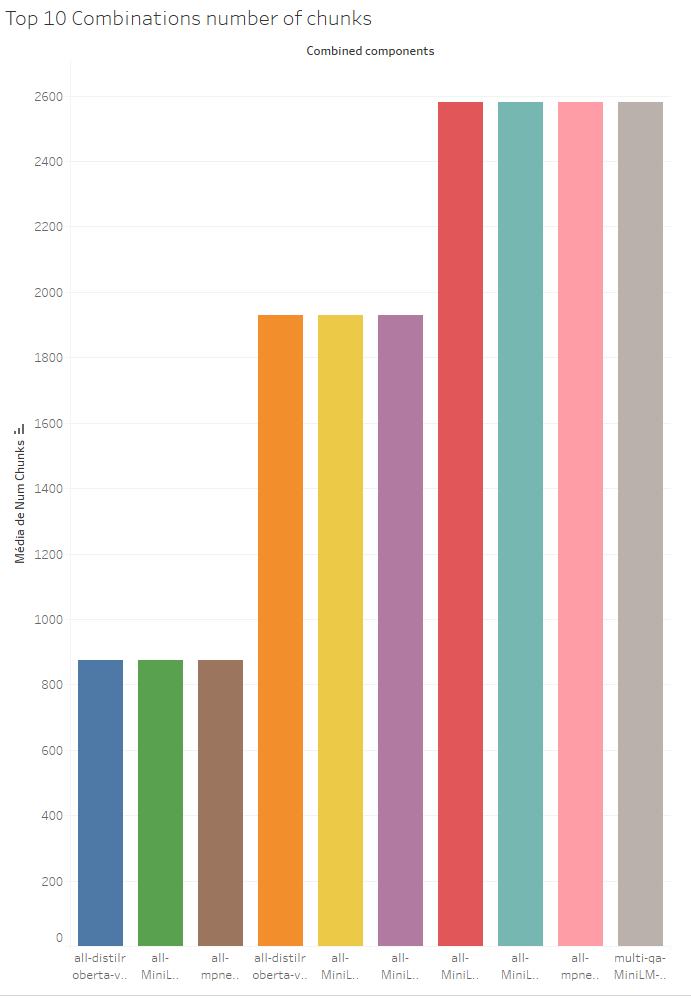
\includegraphics[width=0.6\linewidth]{Chapters/Figures/number_of_chuncks.png}
    \caption{Number of chunks created by each top 10 configurations}
\end{figure}

\begin{figure}[htbp]
    \centering
    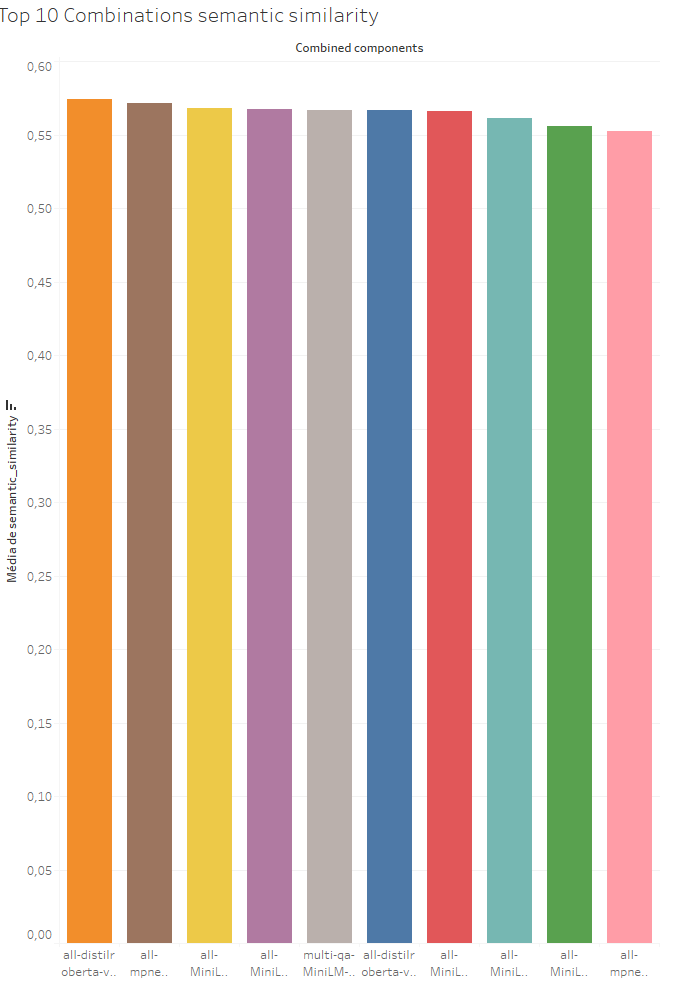
\includegraphics[width=0.6\linewidth]{Chapters/Figures/semantic_similarity.png}
    \caption{Semantic similarity score of the top 10 configuration}
\end{figure}

\textbf{MMR-based retrievers consistently outperformed} others, especially when paired with MiniLM or multi-qa embeddings.

\textbf{Ensemble and threshold-based retrievers underperformed}, especially in recall-heavy queries like class relationships and documentation. Despite theoretical robustness, they introduced inconsistency.

\texttt{multi-qa-MiniLM-L6-cos-v1} and \texttt{all-MiniLM-L6-v2} emerged as the best overall embedding models, appearing repeatedly in the top 3 combinations.

\textbf{Retrieval time and relevance} showed a \textbf{moderate positive correlation} — slower retrievals tended to return more relevant chunks, suggesting a trade-off worth tuning based on latency needs.

\begin{figure}[htbp]
    \centering
    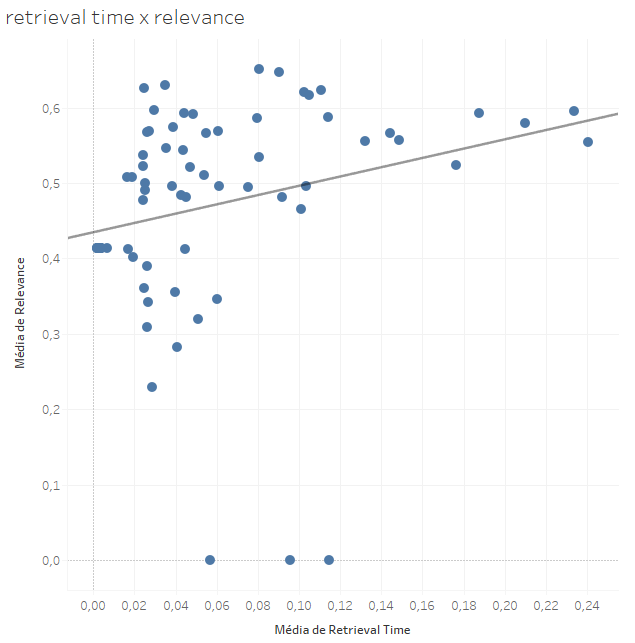
\includegraphics[width=0.6\linewidth]{Chapters/Figures/retrieval_per_relevance.png}
    \caption{Overall benchmark summary.}
\end{figure}

The benchmark shows that the configuration using \texttt{multi-qa-MiniLM-L6-cos-v1}, the default recursive splitter (chunk size = 300), and MMR ($k = 3$, fetch\_k = 10) delivers the \textbf{most balanced performance}, combining strong relevance, accuracy, and efficiency.

Despite small differences in overall scores among the top 10, this configuration stands out due to its ability to scale with a low retrieval time, high semantic coherence, and robust accuracy — making it a strong candidate for production-level UML and PlantUML class diagram understanding tasks.

\section{Self-improve approach}
\label{sec:selfImproveApproach}


Inspired by the iterative refinement framework proposed by Madaan et al.~\cite{madaan2023selfrefineiterativerefinementselffeedback}, this study implements a self-refinement loop in which the same large language model (LLM) is responsible for \textbf{generating}, \textbf{evaluating}, and \textbf{refining} UML class diagrams in an autonomous and cyclical manner. Figure~\ref{fig:self_refinement_loop} illustrates the self-refinement loop.

To prevent excessive or redundant refinement, we impose an upper bound of \textbf{three iterations} per cycle. This decision is empirically supported by the findings of Madaan et al., who observed that while performance improves substantially during the initial two iterations, subsequent iterations tend to yield diminishing returns in both quality and novelty. In addition to this upper limit, we also introduce a \textbf{dynamic stopping condition}: if the improvement in the evaluation score between the current and the previous iteration falls below a threshold of \textbf{0.01}, the loop is terminated early. This ensures that API calls are cost-efficient and only meaningful refinements are performed.

Furthermore, to enhance consistency and reduce redundancy across iterations, we incorporate \textbf{conversational memory} into the prompt context. The model is provided with the content of the two most recent interactions (both the prompt and the corresponding output). This addition was empirically motivated: during initial experimentation, we observed that including minimal conversational history significantly improved the model's ability to avoid previously made errors and reduced the likelihood of introducing redundant or contradictory modifications. However, this improvement in performance comes at the cost of a slightly increased token consumption per API call.

To structure the interactions with the model throughout the self-refinement loop, we adopt a \textbf{Chain-of-Thought (CoT) prompting strategy}~\cite{wei2023chainofthoughtpromptingelicitsreasoning}, which encourages the model to reason through tasks step by step. Each of the three system prompts---\textbf{generation}, \textbf{evaluation}, and \textbf{improvement} was carefully engineered to align with the cognitive role expected of the model during its respective task.

\begin{itemize}
    \item The \textbf{generation prompt} is framed in a descriptive and procedural tone. It guides the model step-by-step through the tasks of entity identification, relationship analysis, attribute extraction, application of UML design principles, and final validation. (can be seen in Listing~\ref{lst:generation_prompt})
    \item The \textbf{evaluation prompt} adopts a formal and analytical tone, simulating the role of an academic reviewer or UML expert. It instructs the model to assess the class diagram against a rubric of weighted criteria. (can be seen in Listing~\ref{lst:improvement_prompt})
    \item The \textbf{improvement prompt} takes on a mentor-like tone, instructing the model to act as a senior software architect improving a junior designer's work. (can be seen in Listing~\ref{lst:evaluation_prompt})
\end{itemize}

\begin{figure}[htbp]
    \centering
    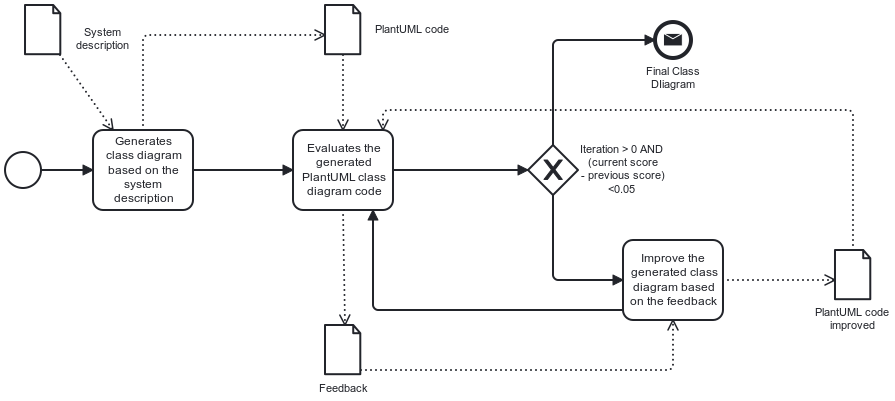
\includegraphics[width=0.8\textwidth]{Chapters/Figures/self-refinement.png}
    \caption{Self-refinement loop architecture.}
    \label{fig:self_refinement_loop}
\end{figure}

\subsubsection{Generation Prompt}

\begin{lstlisting}[caption={Generation Prompt},label={lst:generation_prompt}]

You're a practical and experienced software architect. Your job is to translate a system description into a clean, readable, and syntactically correct PlantUML class diagram. Focus on clarity, correctness, and matching the described system as directly as possible.

## Step by Step to create a class diagram

### Step 1: Entity Identification
- Identify Nouns: Extract all significant nouns from the requirements
- Classify Entities: Categorize as concrete classes, abstract classes, or interfaces
- Eliminate Redundancies: Remove duplicate or overly similar concepts

### Step 2: Relationship Analysis
- Identify Associations: Look for "has-a", "uses", "manages", "contains" relationships
- Determine Inheritance: Find "is-a" relationships and generalization hierarchies
- Establish Multiplicity: Always specify multiplicities (e.g., "1" *-- "1..*")
- Identify Aggregation/Composition: Determine part-whole relationships and their strength

### Step 3: Attribute and Method Extraction
- Extract Attributes: Identify properties each class should contain
- Determine Methods: Identify behaviors and operations
- Apply Encapsulation: Consider visibility modifiers

### Step 4: UML Principles Application
- Single Responsibility, Cohesion, Coupling, Abstraction

### Step 5: Validate & Refine
- Ensure no PlantUML syntax errors
- All requirements mapped

## PlantUML Syntax Guidelines
[class declarations, relationships, multiplicities, stereotypes...]

## Output Requirements
1. Begin with @startuml and end with @enduml
2. Use PascalCase for classes, camelCase for attributes/methods
3. Group related classes logically
4. Include relationship labels and multiplicities
5. Represent all significant entities and relationships


user_prompt = "Generate a class diagram based on the following system description:\n **System Description**\n" + system_description + "\n"
\end{lstlisting}

\subsubsection{Improvement Prompt}

\begin{lstlisting}[caption={Improvement Prompt},label={lst:improvement_prompt}]

You're an experienced software design mentor reviewing a junior architect's class diagram. You've received feedback that highlights issues, and your job is to revise it accordingly.

## Your Task
Analyze the provided feedback and systematically improve the class diagram while maintaining the original requirements.

## Improvement Guidelines
1. UML Completeness: Add missing classes, attributes, relationships
2. UML Quality: Fix naming conventions, relationship types, multiplicities
3. Requirement Coverage: Ensure all requirements are modeled
4. Clarity: Improve labels, organize classes, add stereotypes

## Output Instructions
- Provide complete improved PlantUML diagram
- Start with @startuml and end with @enduml
- Address ALL issues and recommendations
"""

improve_user_prompt = f"""
Improve the following PlantUML class diagram based on the following feedback:
## Current Diagram
{current_response}

## Feedback
{json.dumps(feedback.get('feedback', ''), indent=2)}

## Issues
{chr(10).join(f"- {issue}" for issue in feedback.get('issues', []))}

## Recommendations
{chr(10).join(f"- {rec}" for rec in feedback.get('recommendations', []))}

\end{lstlisting}

\subsubsection{Evaluation Prompt}

\begin{lstlisting}[caption={Evaluation Prompt},label={lst:evaluation_prompt}]

You are acting as a formal academic reviewer with expertise in software architecture and modeling.

## Evaluation Framework
1. UML Completeness (25%)
2. UML Quality (25%)
3. Requirement Coverage (30%)
4. Clarity & Pragmatics (20%)

Each scored 0.0-1.0 with detailed criteria.

## Output Format (JSON)
{
  "uml_completeness_score": <float>,
  "uml_quality_score": <float>,
  "requirement_coverage_score": <float>,
  "pragmatic_clarity_score": <float>,
  "overall_score": <float>,
  "detailed_analysis": {...},
  "issues": [...],
  "recommendations": [...],
  "strengths": [...]
}

Overall score = (completeness*0.25)+(quality*0.25)+(coverage*0.30)+(clarity*0.20)

\end{lstlisting}

\section{Automatic Modelation pipeline using system description}
\label{sec:automatic_modelation_pipeline}
To operationalize the pipeline, we integrate all developed components into a coherent architecture. As illustrated in Figure~\ref{fig:all_system}, the system is composed of three main modules, each responsible for a distinct phase of the process.

\begin{figure}[htbp]
    \centering
    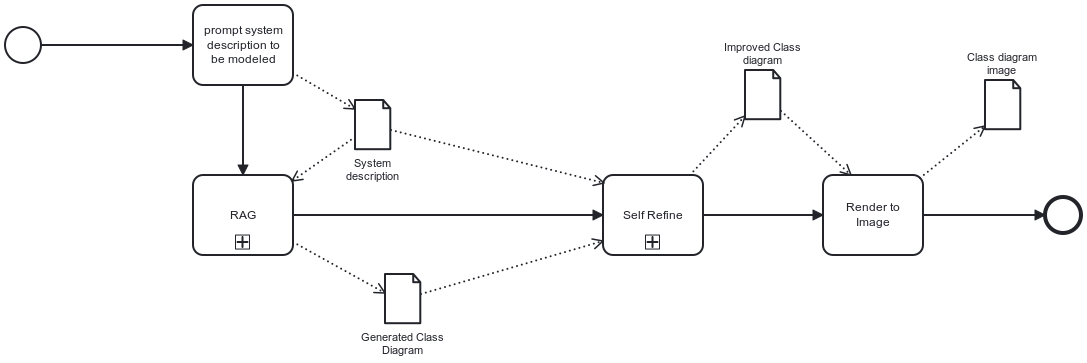
\includegraphics[width=0.8\textwidth]{Chapters/Figures/AllSystem.png}
    \caption{Overall architecture of the proposed system.}
    \label{fig:all_system}
\end{figure}

With all components developed, we now integrate them into a unified system. As illustrated in Figure~\ref{fig:all_system}, the architecture is composed of three main modules:
\begin{enumerate}
    \item \textbf{Generation Module} - Responsible for producing the initial class diagram using a Retrieval-Augmented Generation (RAG) system;
    \item \textbf{Refinement Module} - Refines the initial diagram based on self-evaluation;
    \item \textbf{Rendering Module} - Converts the PlantUML code into a PNG image for visualization.
\end{enumerate}

In the final implementation, we adopt a distinctive RAG approach. Instead of directly using the system description as the query for retrieval, we utilize a predefined set of domain-specific questions to extract relevant knowledge chunks from our database. These questions, along with the retrieved content, are passed to the Haiku~3 model, which generates natural language responses. These responses then serve as contextual input for the prompt that generates the initial class diagram from the system description. This modular and context-enriched strategy is extensible to other types of UML diagrams beyond class diagrams.

Once the PlantUML code for the class diagram is generated, the system proceeds to refine it. The refinement process follows the methodology and prompt design described in the previous section, leveraging self-evaluation and iterative improvement strategies.

After refinement, the final PlantUML code is saved with a unique identifier and rendered into a PNG image using the official PlantUML JAR tool. The resulting diagram is then presented to the user via the interface.

\section{Challenges}
\label{sec:challenges}
This section outlines the main challenges encountered during the development of the system, along with the strategies employed to address them.

\subsection{Cost Reduction in LLM API Usage}

The use of commercial Large Language Model (LLM) APIs, such as Anthropic’s Claude models, entails operational costs. These are typically calculated based on the number of input and output tokens per request, with pricing varying by model (e.g., Claude 3 Haiku vs.\ Claude 3 Opus).

To balance performance and cost-efficiency, we conducted preliminary experiments (see ``Prompt Technique and Model Used'' section) to identify a model that provided satisfactory results while maintaining a lower cost per call. Haiku 3 and 3.7 Sonnet emerged as viable options due to their relatively low pricing and competitive performance.

In addition, we implemented several mitigation strategies:
\begin{itemize}
    \item \textbf{Prompt Optimization}: Prompts were crafted to be concise, retaining only essential information. This reduced the input token count while preserving effectiveness.
    \item \textbf{Structured Output Specification}: We explicitly defined the desired output format (e.g., JSON or PlantUML) within the prompt. This constrained the response length and improved consistency, which in turn minimized the number of output tokens.
\end{itemize}

These techniques collectively contributed to the reduction of total API usage costs without significantly compromising generation quality.

\subsection{Selecting and Configuring RAG Components}

The construction of a Retrieval-Augmented Generation (RAG) system involves a wide variety of configurable components---including chunking strategies, embedding models, retrievers, and re-ranking methods. Given the combinatorial nature of these options, identifying the optimal configuration posed a significant challenge.

To manage this complexity, we adopted a pragmatic approach:
\begin{itemize}
    \item \textbf{Scope Limitation}: Rather than testing the full spectrum of RAG architectures, we focused on implementing a basic (or ``naive'') RAG pipeline.
    \item \textbf{Use of Open-Source Tools}: We prioritized open-source and freely available components to ensure cost-efficiency and reproducibility.
    \item \textbf{Empirical Evaluation}: From the pool of commonly adopted tools (e.g., HuggingFace Transformers, FAISS, and Chroma), we selected the most widely used and tested them across different configurations.
\end{itemize}

By narrowing the scope and selecting community-supported tools, we were able to reduce implementation complexity while still conducting meaningful evaluations.


\section{Pratical Demonstration}
\label{sec:praticalDemonstration}\
In this section we present our proposed system and show its feasibility by applying it to a realistic use case, demonstrating how our automatic process can be applied to a system description and examining the results.

For this proof of concept, we used a system description of a Patient Record and Scheduling system present in the database (referência à base de dados). The description can be found in Listing~\ref{lst:patient_system}.

\begin{lstlisting}[caption={System Description: Patient Record and Scheduling System},label={lst:patient_system}]
A patient record and scheduling system in a doctor's office is used by the receptionists, nurses, and doctors. The receptionists use the system to enter new patient information when first-time patients visit the doctor. They also schedule all appointments. The nurses use the system to keep track of the results of each visit including diagnosis and medications. For each visit, free form text fields are used to capture information on diagnosis and treatment. Multiple medications may be prescribed during each visit. The nurses can also access the information to print out a history of patient visits. The doctors primarily use the system to view patient history. The doctors may enter some patient treatment information and prescriptions occasionally, but most frequently they let the nurses enter this information. -- Each patient is assigned to a family. The head of family is responsible for the person with the primary medical coverage. Information about doctors is maintained since a family has a primary care physician, but different doctors may be the ones seeing the patient during the visit.
\end{lstlisting}

\begin{figure}[htbp]
    \centering
    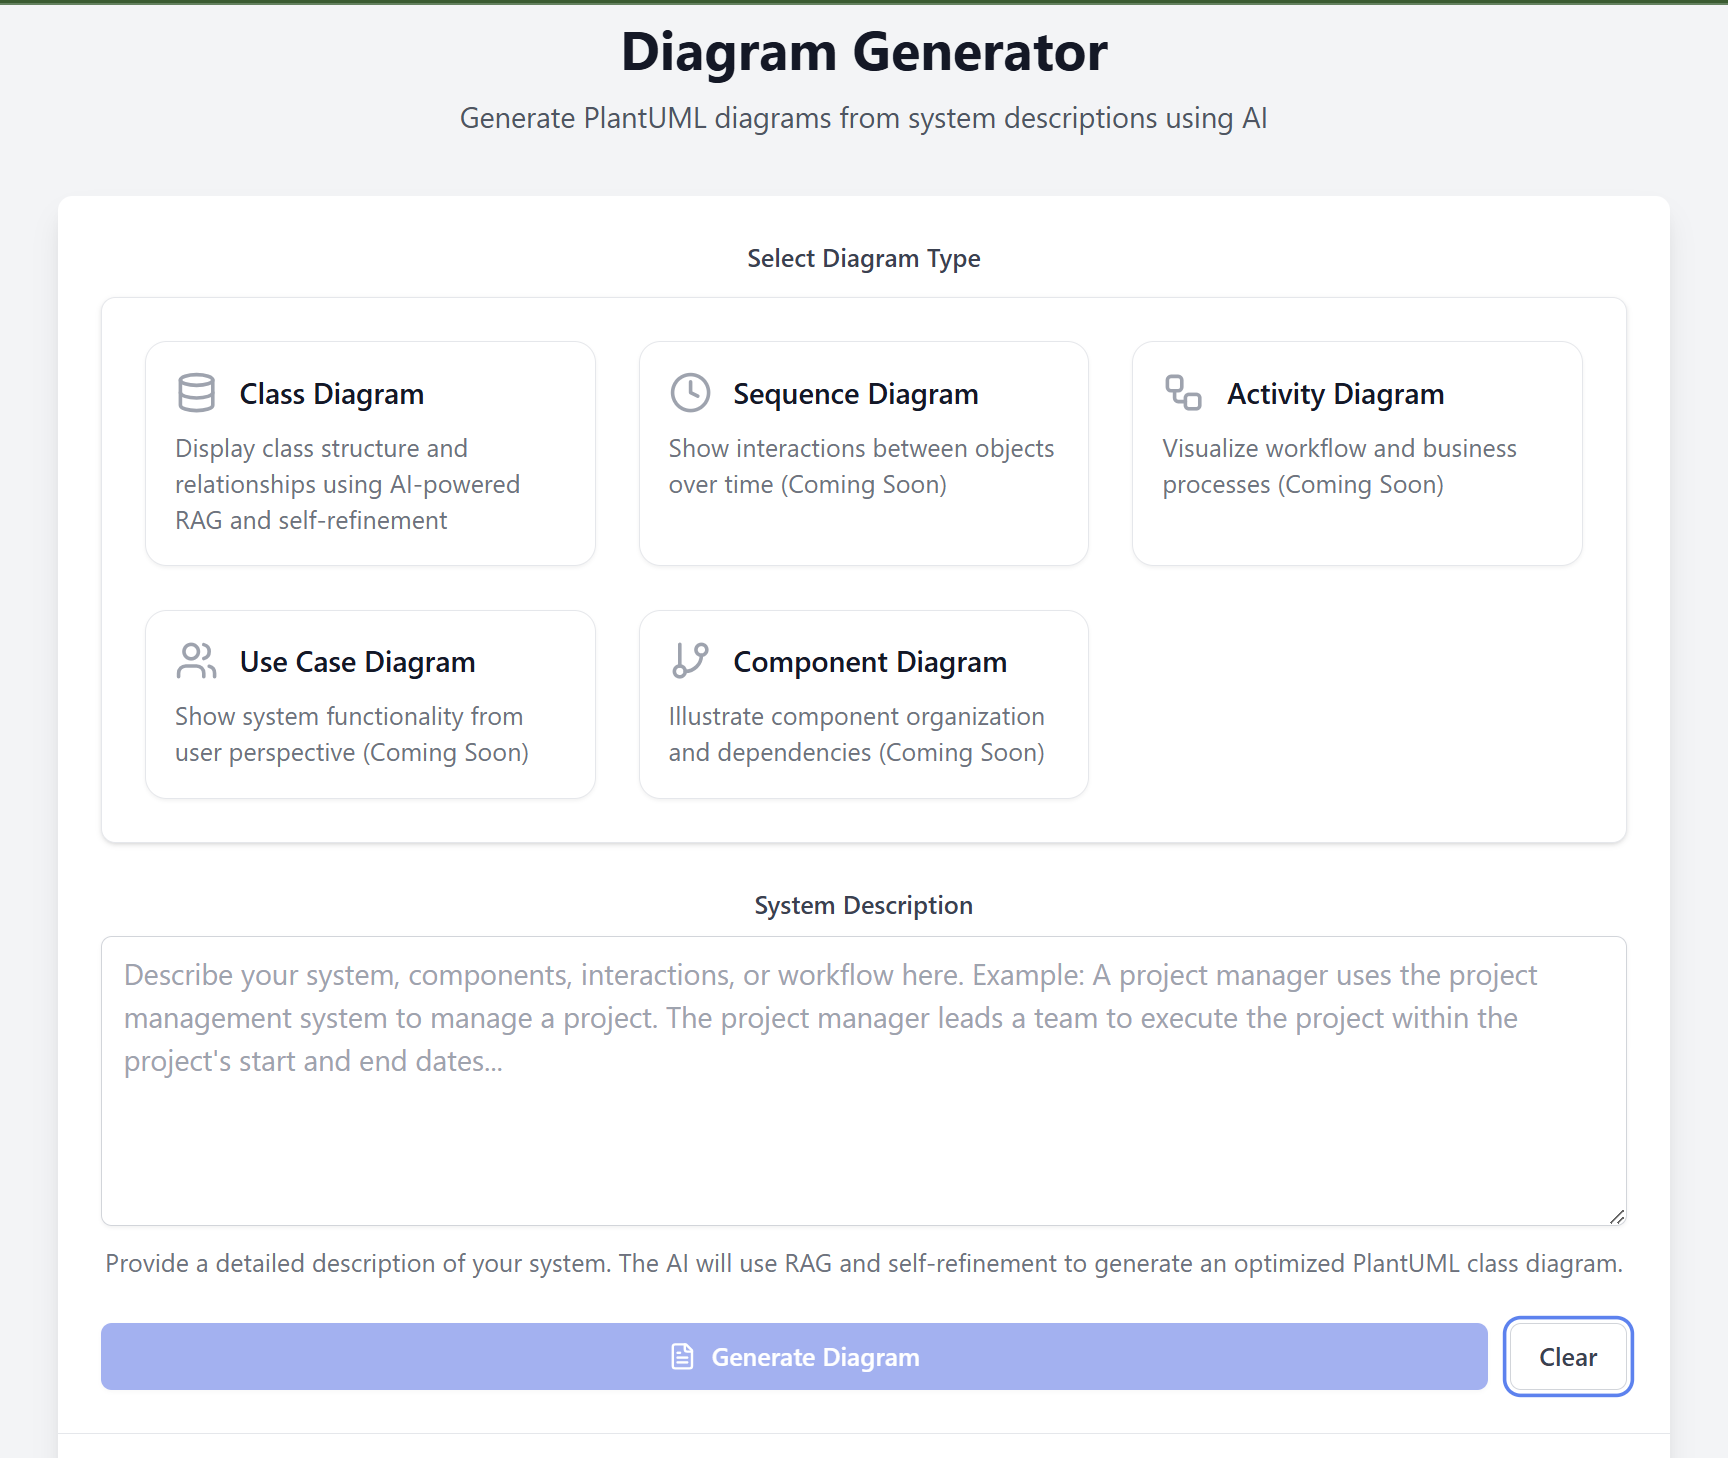
\includegraphics[width=0.8\textwidth]{Chapters/Figures/Interface.png}
    \caption{System interface for the use case}
    \label{fig:patient_system_interface}
\end{figure}

For a better understanding of the execution of the transformation approach, the following steps describe the events leading to the final diagram:

\begin{enumerate}
    \item The user selects the type of diagram to generate.
    \item The user describes the system in the text box.
    \item The user clicks on the button to generate the diagram.
    \item The frontend sends a request to generate the diagram.
    \item The user waits between 30 and 60 seconds.
    \item After generation, the user can save the image and view the corresponding PlantUML code.
\end{enumerate}

The result can be seen in Figure~\ref{fig:ai_result}, compared to the ground truth diagram in Figure~\ref{fig:ground_truth}.

\begin{figure}[h]
    \centering
    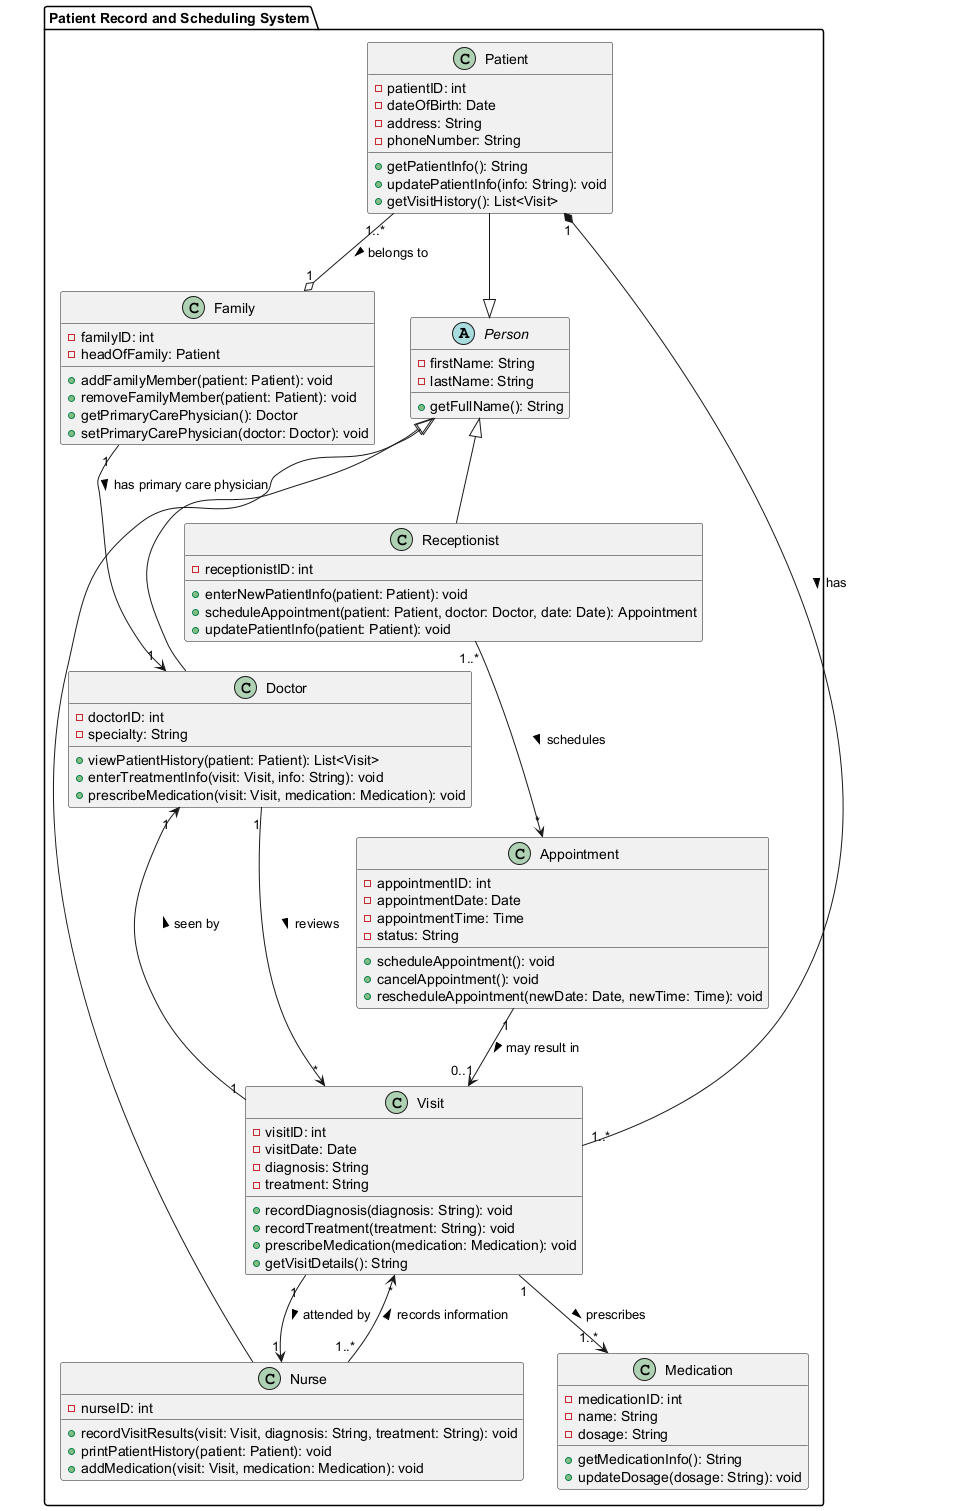
\includegraphics[width=0.8\textwidth]{Chapters/Figures/result_diagram.png}
    \caption{AI-generated class diagram}
    \label{fig:ai_result}
\end{figure}

\begin{figure}[h]
    \centering
    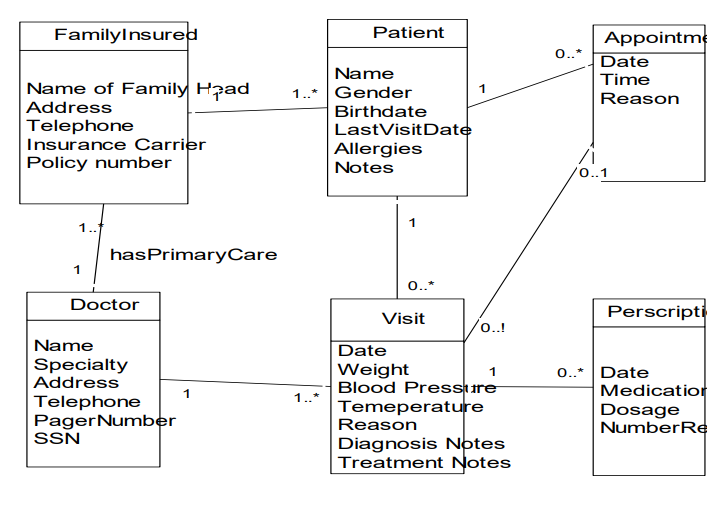
\includegraphics[width=0.8\textwidth]{Chapters/Figures/benchmark.png}
    \caption{Ground truth class diagram}
    \label{fig:ground_truth}
\end{figure}

The generated class diagram includes the set of core domain concepts (Patient, Visit, Appointment, Doctor, Medication and Family) present in the system description. Besides these core concepts, also identified in the ground truth, it includes classes to represent the nurse workers and the receptionists, both mentioned in the system description and associated with functional requirements.

It introduces an abstract Person class, which Patient and Receptionist inherit from. This ensures that shared details such as names and contact information are only defined once, avoiding duplication and making the design easier to maintain. It also adds more specific roles like Nurse and Receptionist, which were not included in the ground truth diagram. This helps to more accurately model the actual roles and responsibilities within a healthcare setting.

With respect to multiplicities, the application attempts to capture the requirement that “multiple medications may be prescribed during each visit.” However, representing this as a direct Visit--Medication association is imprecise. The ground-truth diagram is stronger here: it introduces a Prescription association object that links a Visit to a Medication and carries visit-specific data (e.g., dosage, refills). This design correctly supports the multiplicities Visit 1 -- 0.. Prescription and Prescription 0.. -- 1 Medication, and prevents dosage from being incorrectly modeled as a property of the medication itself.

Regarding relationships, the AI-generated diagram is clearer than the ground truth: instead of just showing a line, it labels relationships with descriptive names such as ``has primary care physician'' or ``attended by''. It even models real-world scenarios more closely, such as an Appointment possibly leading to a Visit.

The AI diagram also goes beyond the specification by adding numerous operations (e.g., scheduling, cancelling appointments, getters). This can be useful in software design by adding more detail to the model.

In summary, compared with the ground truth, the principal deficiency of the AI-generated diagram is the absence of a dedicated Prescription class. Despite this, the diagram is more complete, uses class hierarchies to avoid redundancy, and includes more realistic workflows. In short, while the ground truth contains the basic concepts of the system, the AI-generated diagram represents a more functional and detailed design, making it a stronger blueprint for actual system implementation.

\section{Summary}
This chapter presented the proposed approach for automating UML class diagram generation from system descriptions. It detailed the selection of the optimal prompt strategy (CoT) and LLM (Claude 3.7 Sonnet) based on empirical evaluation, the design of a lightweight and efficient RAG pipeline, and the implementation of a self-refinement loop for iterative improvement. The complete system architecture integrates generation, refinement, and rendering modules. A practical case study demonstrated the system’s effectiveness, producing diagrams that were more complete and detailed than the ground truth, while highlighting areas for further refinement.